\chapter{Methods}
    \label{cha:methods}
    %
    \section{Chromatin Model}
        %
        The chromatin in \ed is modelled as an array of half-nucleosomes (for simplicity, the the array of half-nucleosomes  is referred to as nucleosome string in the rest of the work), meaning that they only contain a tetramer of H2A, H2B, H3 and H4. The nucleosomes hold their position on the string so that the neighbour relations are fixed. Furthermore, the nucleosomes are reduced to presence or absence of PTMs.
        %

        %
        The model in this work can even be further reduced, that is to a nucleosome containing in most cases 1 ($K27$) single amino acid. In \ref{sec:ResBivalency}, every nucleosome possesses 2 modifiable amino acids, called $K_x$ and $K_y$. All of these amino acids are monoacetylatable as well as monomethylatable. These two modifications are mutually-exclusive.
        %

        %
        The nucleosome string is either modelled to be non-cyclic (as done in \ref{sec:ResNon-cooperative} and \ref{sec:ResNonCyc}) or cyclic (\ref{sec:ResBistableSwitching} to \ref{sec:ResBivalency}). In the cyclic case, the enzymes' context can include nucleosomes from the start as well as the end of the string simultaneously. The non-cyclic models contain 60 nucleosomes whereas the non-cyclic ones only contain 40 nucleosomes.\\
        %
        \begin{itemize}
            {
                \color{red}
                \item limitations
                \item bistability impact on rule set
                \item what starting state?
            }
        \end{itemize}
    %
    %
    % \section{\ed parameters}
    %     %

    % %
    % %
    \section{Enzyme models} % TODO single table? subsections?
        %
        \subsection{Enzymes in \ed}
            %
            \begin{itemize}
                {
                    \color{red}
                    \item context
                    \item rule definition
                    \item only symmetric rules (concerning acetylation and methylation)
                    \item association and reaction+dissociation rates
                    \item side note on concentration depletion
                    \item refer to Gillespie
                    \item either put all the enzyme type reactions in one multifigure or put every type separately, then maybe put the mirrored reactions and/or the methylations
                }
            \end{itemize}
            %
        %
        %
        \subsection{Enzyme types}
            %
            % \begin{figure}[ht!]
            %     \centering
            %     \begin{minipage}{0.6\textwidth}
            %         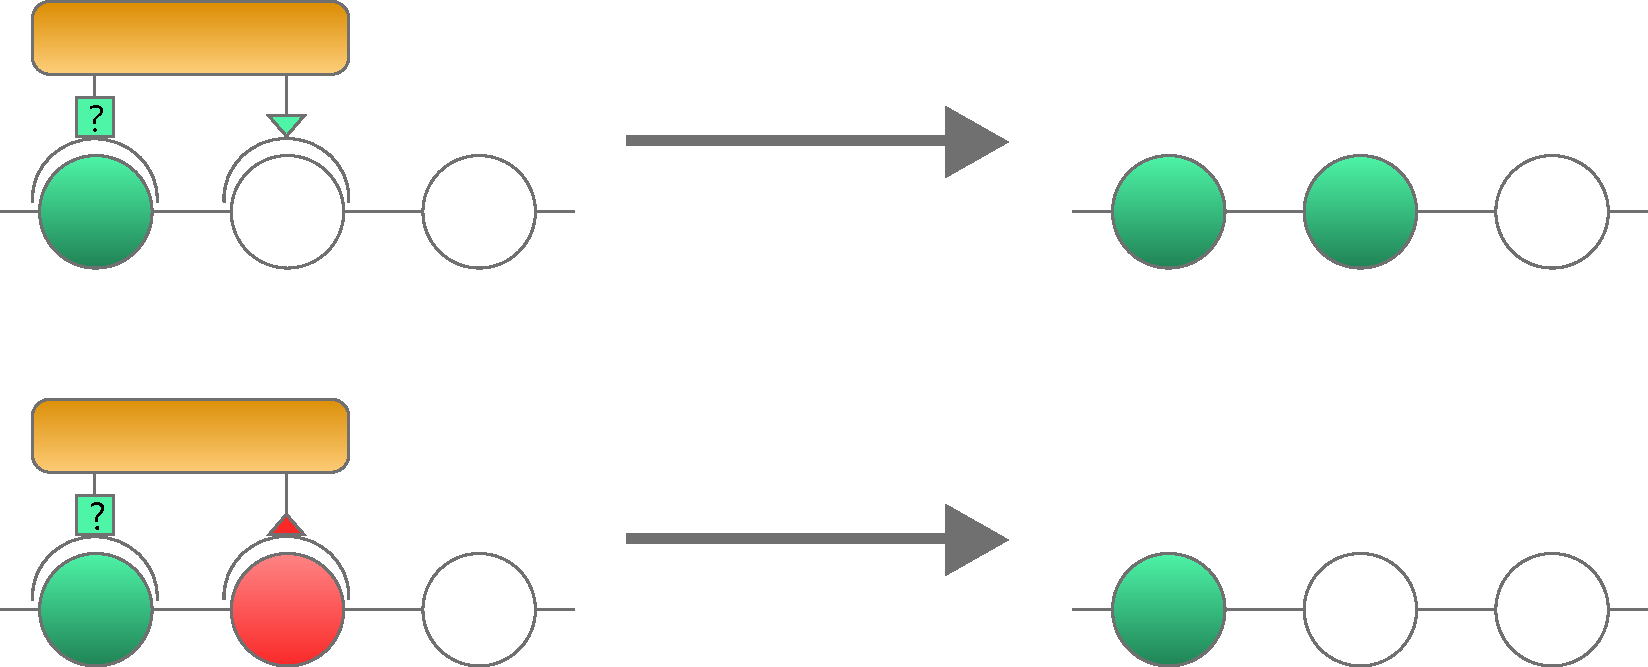
\includegraphics[width=\textwidth]{images/EnzymeModelTest.pdf}
            %         \caption*{\small \textbf{(a)} Linear enzymes}
            %     \end{minipage}
            %     \vspace{1mm}
            %     \begin{minipage}{0.6\textwidth}
            %         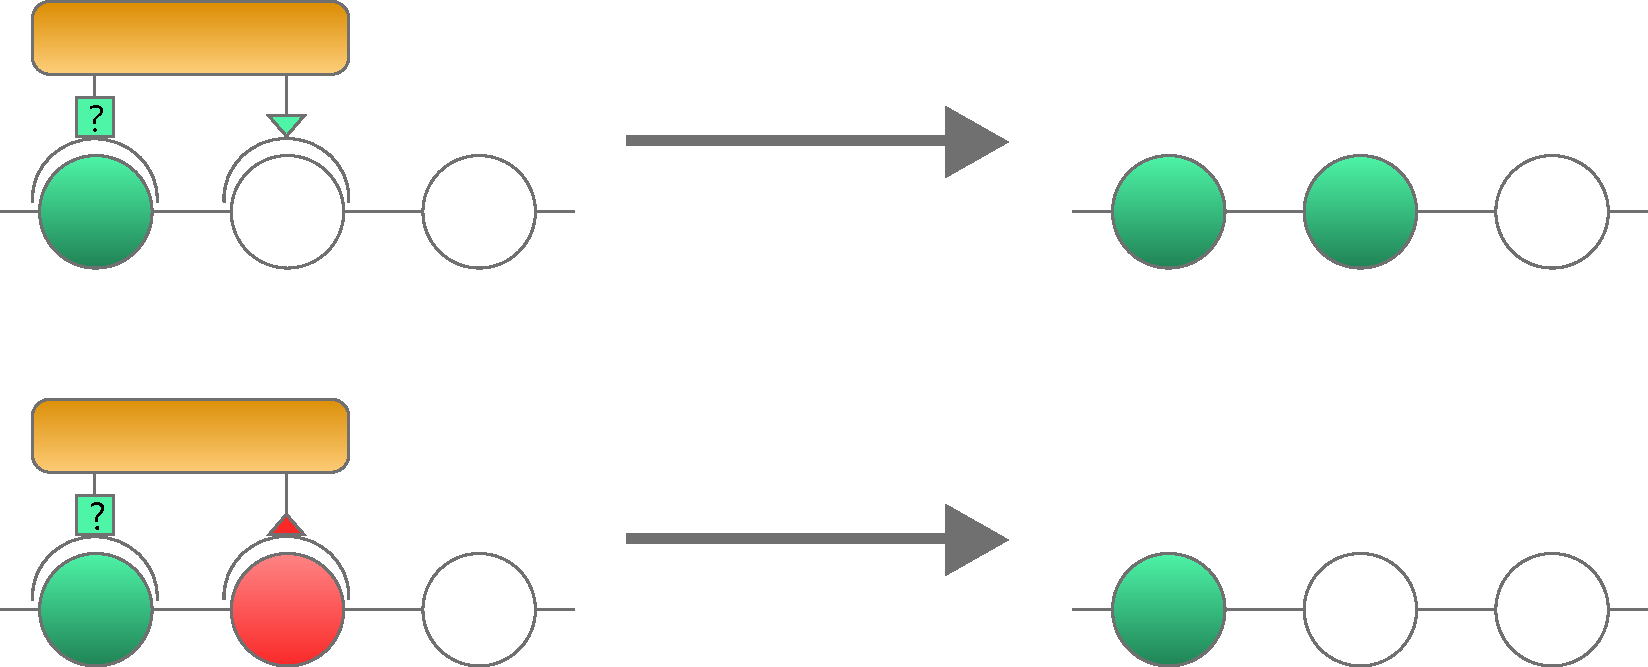
\includegraphics[width=\textwidth]{images/EnzymeModelTest.pdf}
            %         \caption*{\small \textbf{(b)} Cooperative enzymes}
            %     \end{minipage}
            %     \vspace{1mm}
            %     \begin{minipage}{0.6\textwidth}
            %         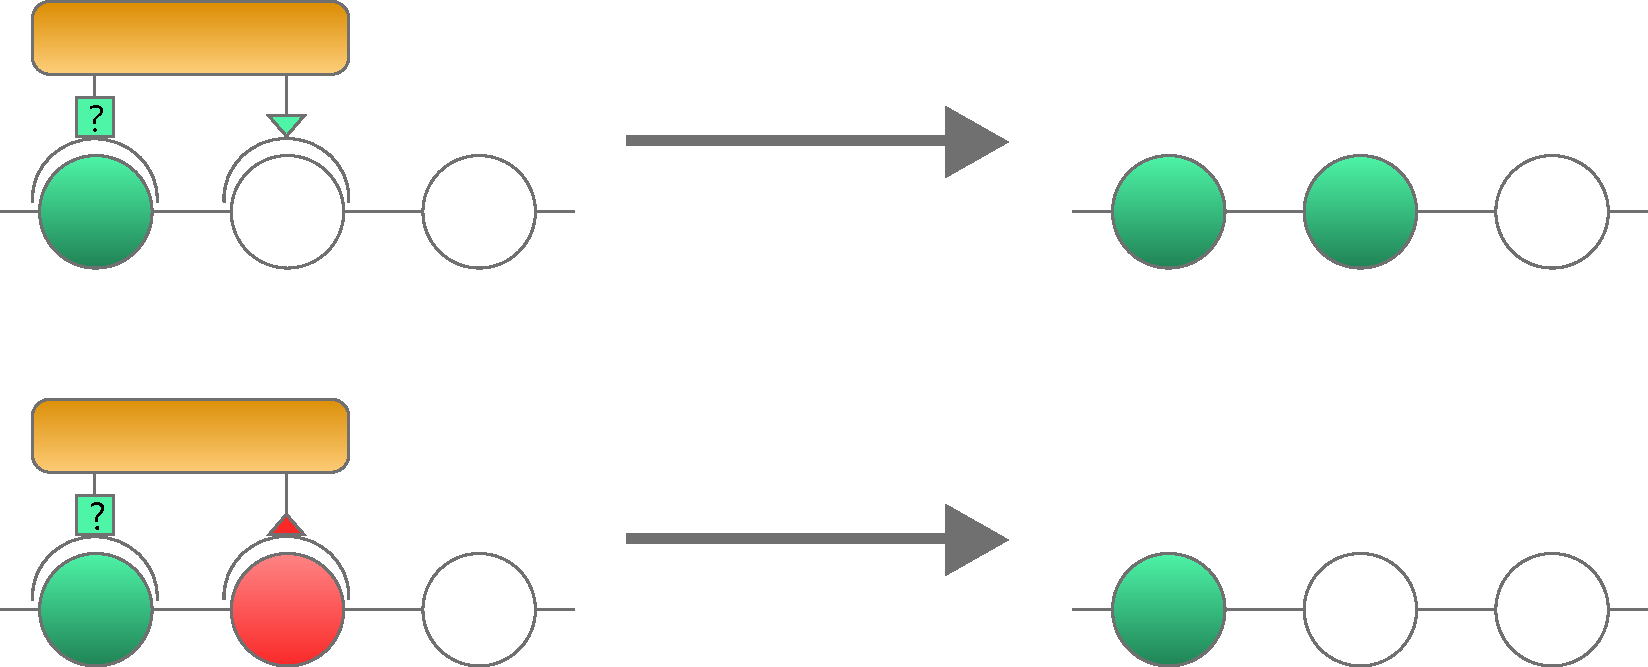
\includegraphics[width=\textwidth]{images/EnzymeModelTest.pdf}
            %         \caption*{\small \textbf{(c)} Random enzymes}
            %     \end{minipage}
            %     \vspace{1mm}
            %     \begin{minipage}{0.6\textwidth}
            %         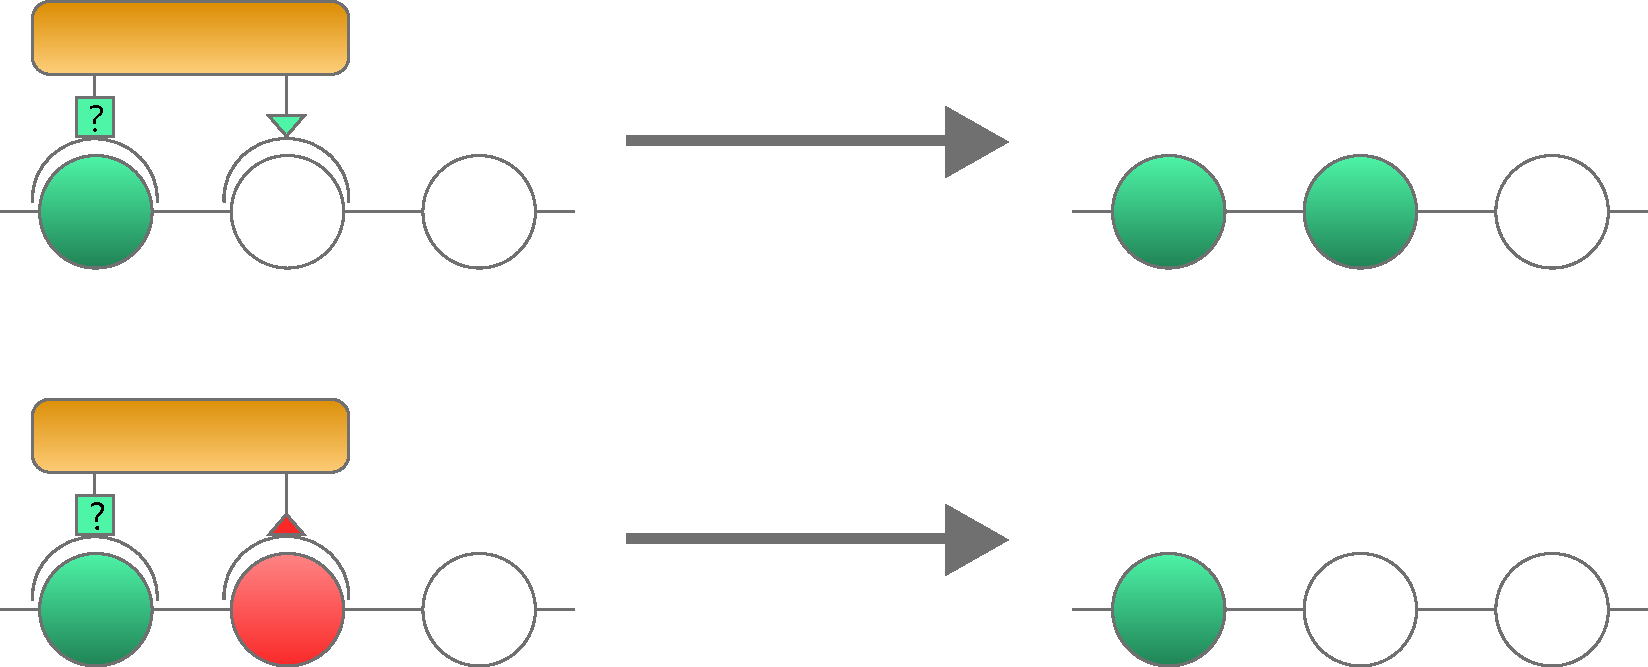
\includegraphics[width=\textwidth]{images/EnzymeModelTest.pdf}
            %         \caption*{\small \textbf{(d)} Completer enzymes}
            %     \end{minipage}
            %    \caption{\small  Graphical depictions of the enzyme types featured in this work and their reactions.  {\color{red} Are the fix points denoted correctly?}}
            %    \label{img:EnzymeTypes}
            % \end{figure}
            %
            \subsubsection*{Linear enzymes}
                %
                \begin{figure}[htpb!]
                    \centering
                    \begin{minipage}{0.91\textwidth}
                        \begin{minipage}{0.1\textwidth}
                            \caption*{\small \textbf{(a)}}
                        \end{minipage}
                        \begin{minipage}{0.8\textwidth}
                            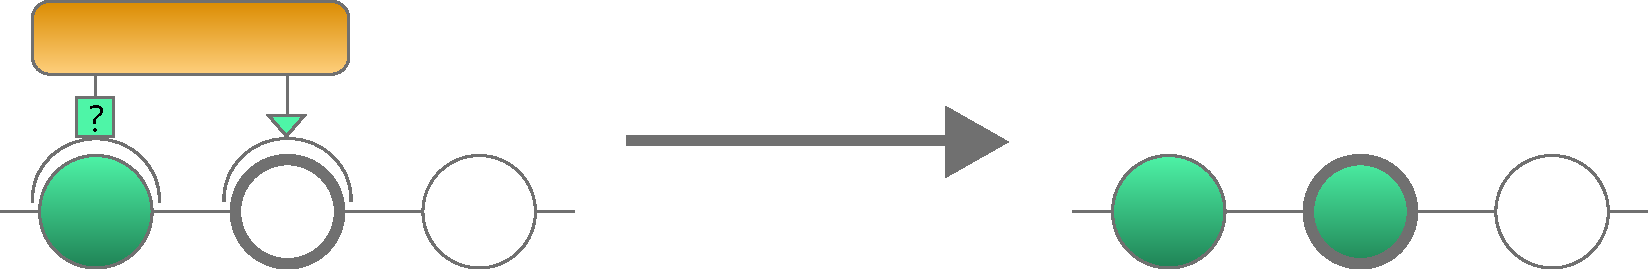
\includegraphics[width=\textwidth]{enzymes/linear_a.pdf}
                        \end{minipage}
                    \end{minipage}
                    \begin{minipage}{0.91\textwidth}
                        \begin{minipage}{0.1\textwidth}
                            \caption*{\small \textbf{(b)}}
                        \end{minipage}
                        \begin{minipage}{0.8\textwidth}
                            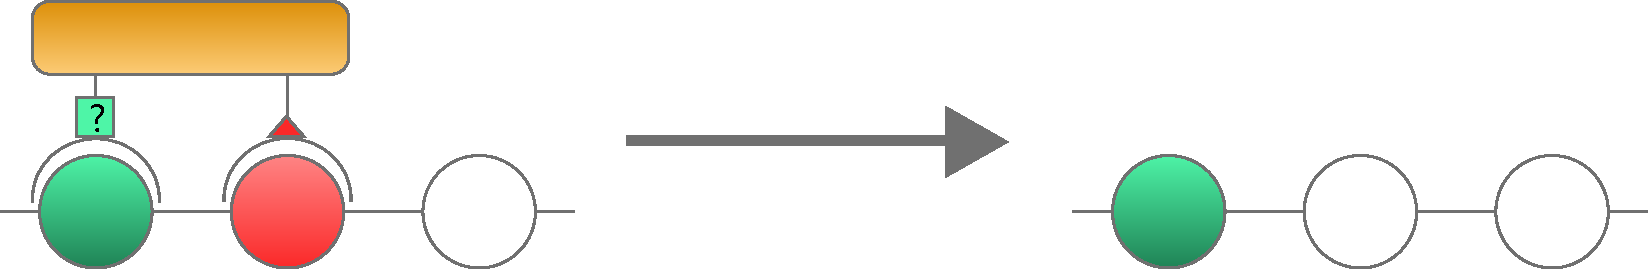
\includegraphics[width=\textwidth]{enzymes/linear_b.pdf}
                        \end{minipage}
                    \end{minipage}
                    \caption{Graphical depiction of the possible linear enzyme acetylation addition \textbf{(a)} and removal \textbf{(b)} reactions. The reactions shown are also defined in the rule set to occur in the opposite direction. Linear enzyme methylators work analogically.}
                    \label{img:linearEnzymes}
                \end{figure}
                %
                Linear enzymes can also be considered next-neighbour enzymes. They are used to extending sites containing a specific modification by either propagating the modification from nucleosome to neighbouring unmodified nucleosome or by deleting an opposing modification next to a nucleosome with the desired modification.
                %
            %
            %
            \subsubsection*{Cooperative enzymes}
                %
                \begin{figure}[htpb!]
                    \centering
                    \begin{minipage}{0.97\textwidth}
                        \begin{minipage}{0.1\textwidth}
                            \caption*{\small \textbf{(a)}}
                        \end{minipage}
                        \begin{minipage}{0.86\textwidth}
                            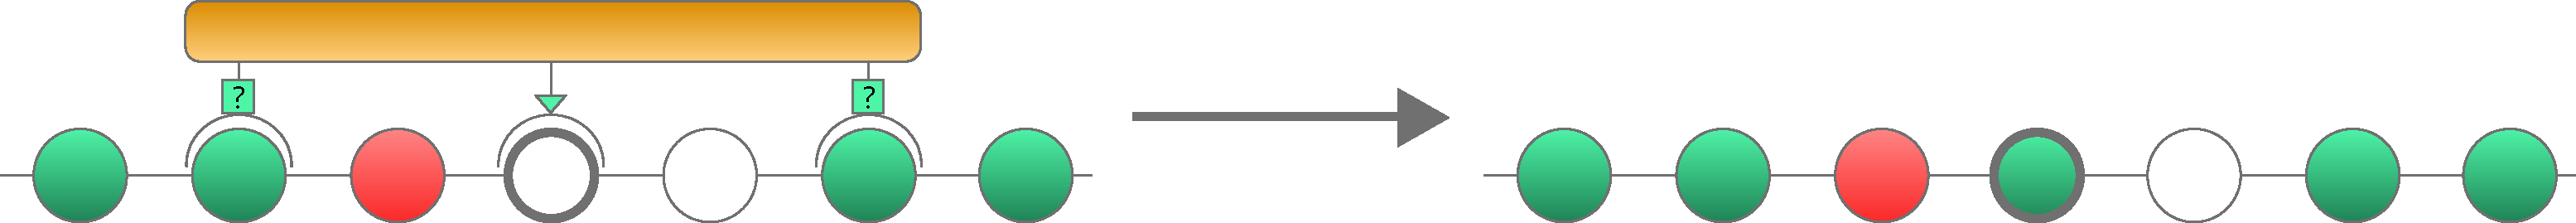
\includegraphics[width=\textwidth]{enzymes/coop_a.pdf}
                        \end{minipage}
                    \end{minipage}
                    \begin{minipage}{0.97\textwidth}
                        \begin{minipage}{0.1\textwidth}
                            \caption*{\small \textbf{(b)}}
                        \end{minipage}
                        \begin{minipage}{0.86\textwidth}
                            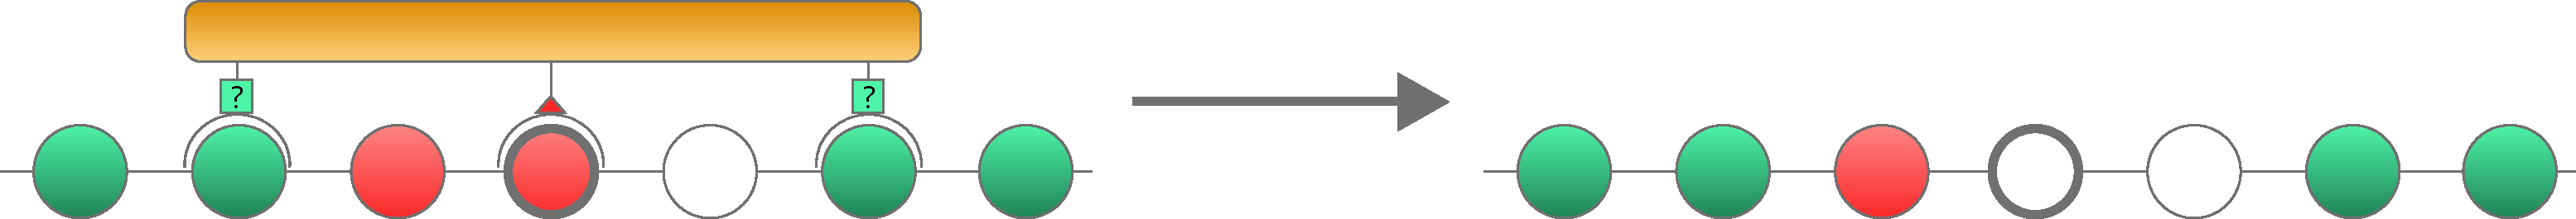
\includegraphics[width=\textwidth]{enzymes/coop_b.pdf}
                        \end{minipage}
                    \end{minipage}
                    \caption{Graphical depiction of the possible cooperative enzyme acetylation addition \textbf{(a)} and removal \textbf{(b)} reactions. The reactions shown are also defined in the rule set to occur in the opposite direction. Cooperative enzyme methylators work analogically.}
                    \label{img:coopEnzymes}
                \end{figure}
                %
                \begin{itemize}
                    {
                        \color{red}
                        \item spacing that is the same on both sides
                        \item difference to linear enzymes
                    }
                \end{itemize}
                %
            %
            %
            \subsubsection*{Random enzymes}
                %
                \begin{figure}[htpb!]
                    \centering
                    \begin{minipage}{0.91\textwidth}
                        \begin{minipage}{0.1\textwidth}
                            \caption*{\small \textbf{(a)}}
                        \end{minipage}
                        \begin{minipage}{0.8\textwidth}
                            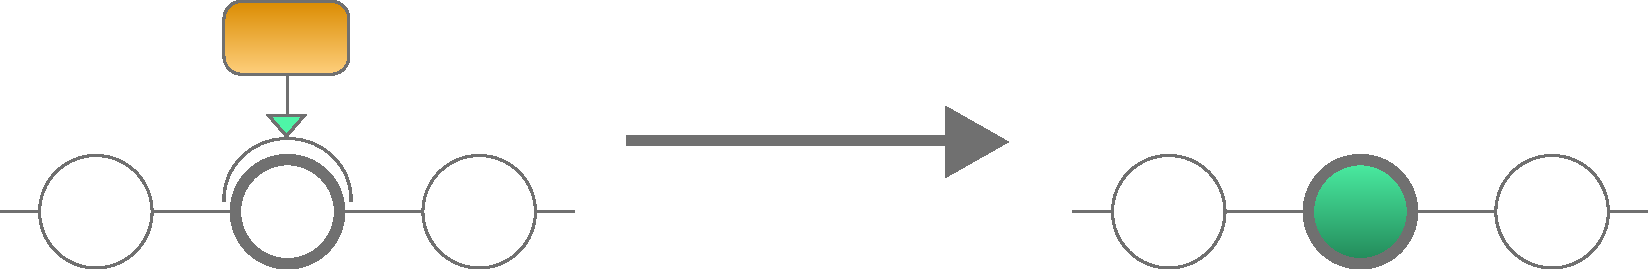
\includegraphics[width=\textwidth]{enzymes/random_a.pdf}
                        \end{minipage}
                    \end{minipage}
                    \begin{minipage}{0.91\textwidth}
                        \begin{minipage}{0.1\textwidth}
                            \caption*{\small \textbf{(b)}}
                        \end{minipage}
                        \begin{minipage}{0.8\textwidth}
                            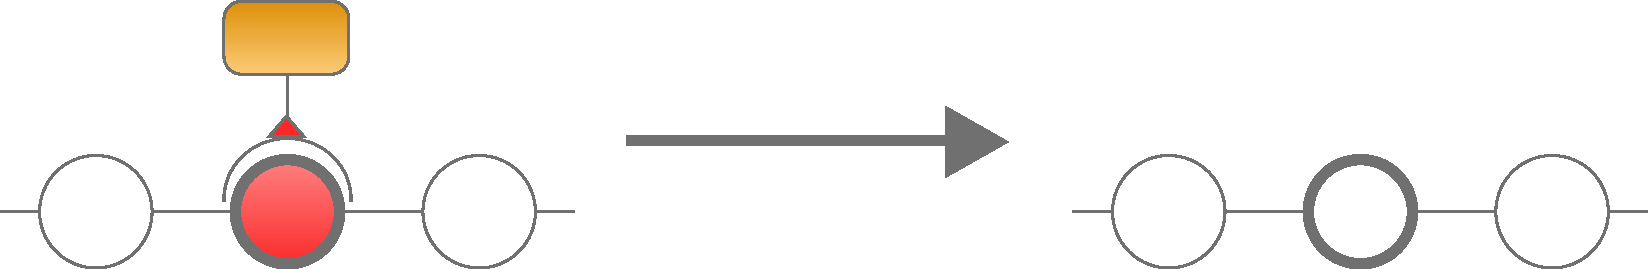
\includegraphics[width=\textwidth]{enzymes/random_b.pdf}
                        \end{minipage}
                    \end{minipage}
                    \caption{Graphical depiction of the possible random enzyme acetylation addition \textbf{(a)} and removal \textbf{(b)} reactions. The reactions shown are also defined in the rule set to occur in the opposite direction. Linear enzyme methylators work analogically.}
                    \label{img:randomEnzymes}
                \end{figure}
                %
                \begin{itemize}
                    {
                        \color{red}
                        \item NOT contextless
                        \item need very low rate (propensity sum)
                        \item bring noise to the system
                        \item not biological as enzymes, but noise is known to be in the system (source?)
                    }
                \end{itemize}
                %
            %
            %
            \subsubsection*{Completer enzymes}
                %
                \begin{figure}[htpb!]
                    \centering
                    \begin{minipage}{0.91\textwidth}
                        \begin{minipage}{0.1\textwidth}
                            \caption*{\small \textbf{(a)}}
                        \end{minipage}
                        \begin{minipage}{0.8\textwidth}
                            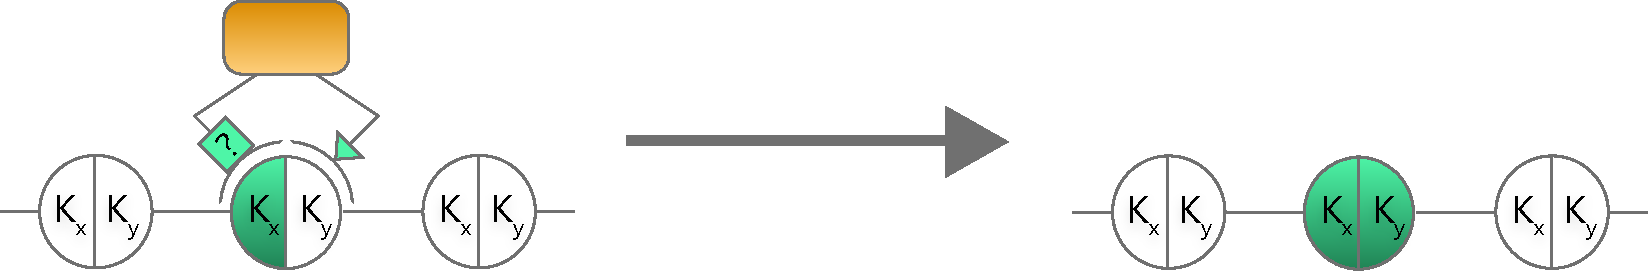
\includegraphics[width=\textwidth]{enzymes/completer_total_a.pdf}
                        \end{minipage}
                    \end{minipage}
                    \begin{minipage}{0.91\textwidth}
                        \begin{minipage}{0.1\textwidth}
                            \caption*{\small \textbf{(b)}}
                        \end{minipage}
                        \begin{minipage}{0.8\textwidth}
                            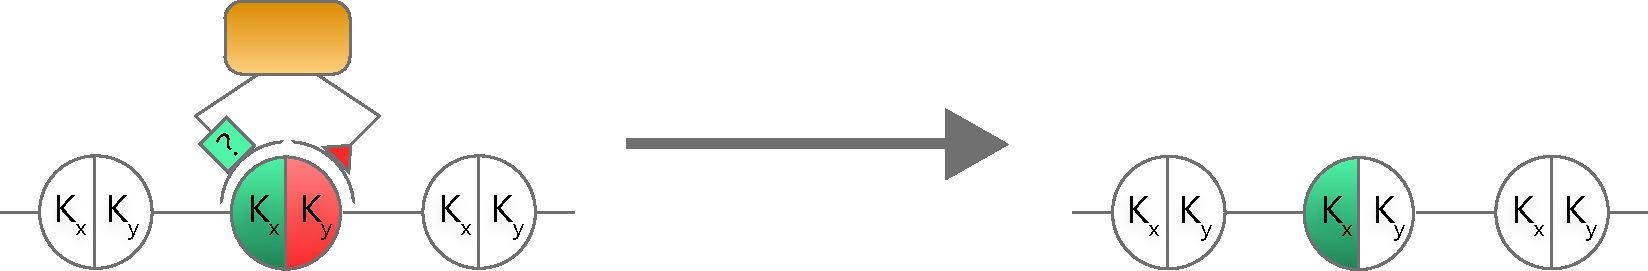
\includegraphics[width=\textwidth]{enzymes/completer_total_b.pdf}
                        \end{minipage}
                    \end{minipage}
                    \begin{minipage}{0.91\textwidth}
                        \begin{minipage}{0.1\textwidth}
                            \caption*{\small \textbf{(c)}}
                        \end{minipage}
                        \begin{minipage}{0.8\textwidth}
                            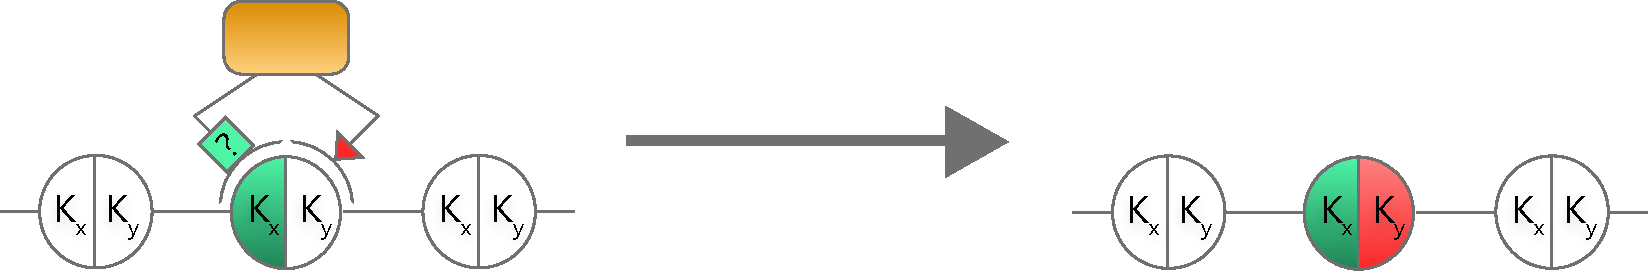
\includegraphics[width=\textwidth]{enzymes/completer_biv_a.pdf}
                        \end{minipage}
                    \end{minipage}
                    \begin{minipage}{0.91\textwidth}
                        \begin{minipage}{0.1\textwidth}
                            \caption*{\small \textbf{(d)}}
                        \end{minipage}
                        \begin{minipage}{0.8\textwidth}
                            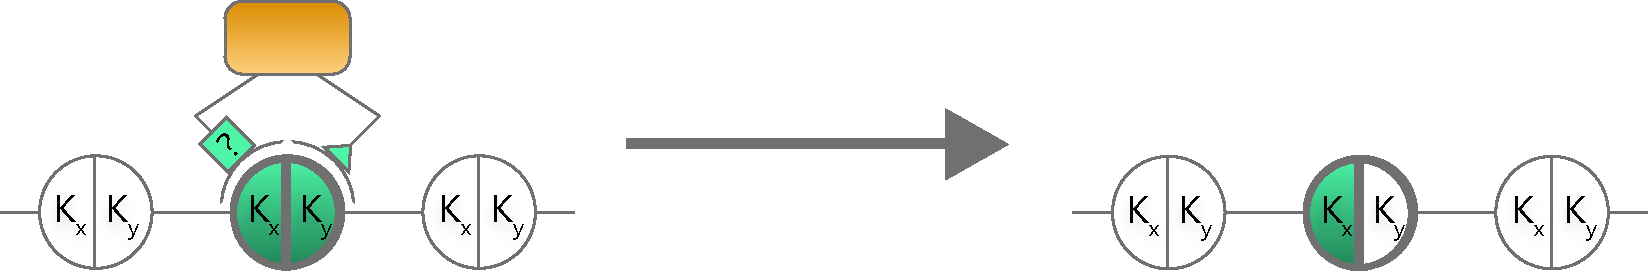
\includegraphics[width=\textwidth]{enzymes/completer_biv_b.pdf}
                        \end{minipage}
                    \end{minipage}
                    \caption{Graphical depiction of the possible total enzyme acetylation addition \textbf{(a)} and removal \textbf{(b)} reactions. The reactions shown are also defined in the rule set to occur in the opposite direction. Total enzyme methylators work analogically.}
                    \label{img:completerEnzymes}
                \end{figure}
                %
                \begin{itemize}
                    {
                        \color{red}
                        \item no known scientific background
                        \item explain Kx Ky model
                    }
                \end{itemize}
                %
            %
            %
        %
        %
        \subsection{Enzyme rule sets}
            %
            \begin{itemize}
                {
                    \color{red}
                    \item Explain the sets later used? and enumerate them or sth so that the reader can easily refer to them. Explain them before.
                }
            \end{itemize}
            \begin{itemize}
                {
                    \color{red}
                    \item 3.1: linear extenders, linear removers, random adders, random removers
                    \item 3.2: cooperative adders, cooperative removers (not for some), random adders, random removers (non-cyclic)
                    \item 3.3: cooperative adders, cooperative removers (not for some), random adders, random removers (cyclic)
                    \item 3.4: cooperative adders, random adders, random removers (cyclic)
                    \item 3.5: cooperative adders, random adders, random removers (cyclic)
                    \item 3.6:
                        \begin{itemize}
                            \item BivalentBistability:
                            \item FavTotal:
                            \item FavBivalency:
                        \end{itemize}
                }
            \end{itemize}
            %
        %
        %
    %
    %
    \section{Simulation parameters/details}
        %
        \begin{itemize}
            {
                \color{red}
                \item How did I change it?
                \item Time setting etc
                \item refer to exemplary state, rule and parameter files in appendix
                \item The simulations are run at two different length categories
                    \begin{itemize}
                        \item short: Every step is plotted to see switching and meta data are used to plot association numbers and relative binding time
                        \item long: Only every 1000th step is plotted. Given that the system is stochastic/chaotic, regular plotting (f. ex. every 1000th data point) results in a smoothing of the histogram because the chosen points are more representative for the underlying distribution.
                    \end{itemize}
            }
        \end{itemize}
        %
    %
    %
%
%